\documentclass[10pt,a4paper]{article}
\usepackage[latin1]{inputenc}
\usepackage[spanish]{babel}
\usepackage{amsmath}
\usepackage{amsfonts}
\usepackage{amssymb}
\usepackage{graphicx}
\usepackage[left=2cm,right=2cm,top=2cm,bottom=2cm]{geometry}
\begin{document}
\section{Marco Te\'{o}rico.}
\textbf{Esfuerzo, deformaci\'{o}n y m\'{o}dulos de elasticidad.}
\\
El cuerpo r\'{i}gido es un modelo idealizado \'{u}til, pero en muchos casos el estiramiento, el aplastamiento y las torsiones de los cuerpos reales cuando se les aplican fuerzas son demasiado importantes para despreciarse. La Figura 1 muestra tres ejemplos. Nos interesa estudiar la relaci\'{o}n entre las fuerzas y los cambios de forma en cada caso.\\ Para cada clase de alteraci\'{o}n de la forma, introduciremos una cantidad llamada \textbf{esfuerzo} que caracteriza la intensidad de las fuerzas que causan el cambio de forma, generalmente con base en la “fuerza por unidad de \'{a}rea. Otra cantidad, \textbf{deformaci\'{o}n}, describe el cambio de forma resultante. Si el esfuerzo y la deformaci\'{o}n son peque\~{n}os, es com\'{u}n que sean directamente proporcionales, y llamamos a la constante de proporcionalidad \textbf{m\'{o}dulo de elasticidad}. Si tiramos con mayor fuerza de algo, se estirar\'{a} m\'{a}s; si lo aplastamos con mayor fuerza, s\'{e} comprimir\'{a} m\'{a}s. El pat\'{o}n general puede formularse as\'{i}:

\\
\[\frac { Esfuerzo }{ Deformaci\'{o}n } =M\'{o}dulo\quad de\quad elasticidad.\quad(Ley\quad de \quad Hooke)\longrightarrow(1)  \]\\

La proporcionalidad del esfuerzo y la deformaci\'{o}n (en ciertas condiciones) se denomina \textbf{ley de Hooke}, en honor a Robert Hooke (1635-1703), un contempor\'{a}neo de Newton. Usamos una forma de la ley de Hooke anteriormente con: el alargamiento de un resorte ideal es proporcional a la fuerza que lo estira. Recordemos que \'{e}sta no es realmente una ley general, sino un resultado experimental v\'{a}lido s\'{o}lo dentro de un intervalo limitado.\\

\\
\begin{figure}[hbtp]
\centering
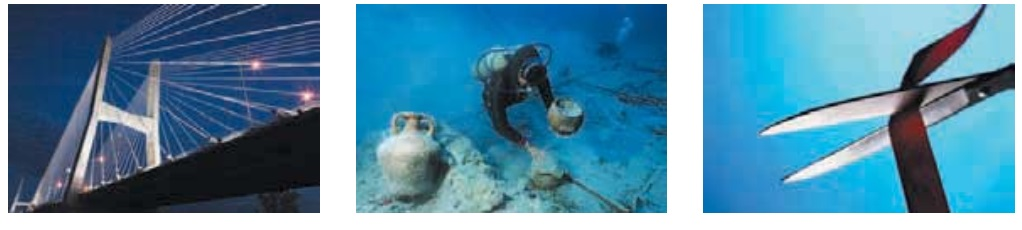
\includegraphics[width=13cm]{../../../../../Pictures/1.jpg}
\caption{Tres tipos de esfuerzos: a) Los cables de un puente sometidos a esfuerzo de tensi\'{o}n, estirados por fuerzas que act\'{u}an en sus extremos. b) Buzo sometido a esfuerzo de volumen, aplastado por todos lados por fuerzas debidas a la presi\'{o}n del agua. c) List\'{o}n sometido a esfuerzo de corte, siendo deformado y finalmente cortado por fuerzas ejercidas por las tijeras.}
\end{figure}
\\


\textbf{ Esfuerzo y deformaci\'{o}n de tensi\'{o}n y compresi\'{o}n.}\\


El comportamiento el\'{a}stico m\'{a}s f\'{a}cil de entender es el estiramiento de una barra, una
varilla o un alambre, cuando se tira de sus extremos (Figura 1.a). La Figura 2
muestra un objeto que inicialmente tiene un \'{a}rea de secci\'{o}n transversal uniforme A y
una longitud lo. Ahora aplicamos fuerzas de igual magnitud $F\bot$  pero direcciones
opuestas a los extremos (esto garantiza que el objeto no tender\'{a} a moverse a la izquierda ni a la derecha).

\begin{figure 2}
\centering
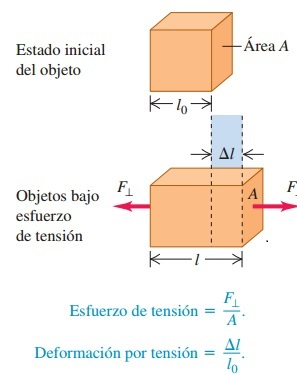
\includegraphics[width=3.4cm]{../../../../../Pictures/2.jpg}
\\
\caption{Figura 2: Un objeto en tensi\'{o}n. La fuerza total que act\'{u}a sobre el objeto es cero, pero el objeto se deforma. El esfuerzo de tensi\'{o}n (la raz\'{o}n de la fuerza al \'{a}rea de secci\'{o}}n transversal) produce una deformaci\'{o}n por tensi\'{o}n (el alargamiento dividido entre la longitud inicial). Por claridad, se ha exagerado el alargamiento .}
\end{figure 2}
\\


Decimos que el objeto est\'{a} en tensi\'{o}n. Ya hablamos mucho de la tensi\'{o}n en cuerdas y cordones; se trata del mismo concepto. \\El sub\'{i}ndice $\bot$ nos
recuerda que las fuerzas act\'{u}an en direcci\'{o}n perpendicular a la secci\'{o}n transversal.
Definimos el esfuerzo de tensi\'{o}n en la secci\'{o}n transversal como el cociente de la
fuerza $F\bot$ y el \'{a}rea de la secci\'{o}n transversal A:\\
\begin{equation}
\[\frac {F\boot}{ A } =Esfuerzo\quad de\quad tensi\'{o}n.\longrightarrow  (2) \]
\end{equation}

\'{E}sta es una cantidad escalar porque $F\bot$ es la magnitud de la fuerza. La unidad del esfuerzo en el pascal (abreviado Pa y as\'{i} llamado en honor del cient\'{i}fico y fil\'{o}sofo franc\'{e}s del siglo XVII Blaise Pascal). La ecuaci\'{o}n anterior muestra que un pascal es igual a 1 newton sobre metro cuadrado (${N}/{ m^{2}} $) :

\\
\[\1\quad Pascal=1pa={ N }/{ { m }^{ 2 } }.\]
\\

En el sistema brit\'{a}nico, la unidad l\'{o}gica del esfuerzo ser\'{i}a la libra por pie cuadrado;
no obstante, es m\'{a}s com\'{u}n utilizar la libra por pulgada cuadrada(${lb}/{in^{2}}$ o psi). Los
factores de conversi\'{o}n son:

\\
\[1\quad psi\quad =\quad 6895\quad Pa\quad y\quad 1 Pa= 1.450{ \times 10 }^{ -4 }psi.\]
\\
Las unidades de esfuerzo son las mismas que las de presi\'{o}n, que veremos a menudo en cap\'{i}tulos posteriores. La presi\'{o}n del aire en los neum\'{a}ticos de un autom\'{o}vil es de alrededor de $3{ \times 10 }^{ -4 }Pa=300kPa$, y normalmente se exige que los cables de acero soporten esfuerzos de tensi\'{o}n del orden de $10^{8}$ Pa. El objeto de la Figura 2 se estira hasta una longitud $l = lo+\Delta l $ cuando se le somete a tensi\'{o}n. El alargamiento $\Delta l$ no se da s\'{o}lo en los extremos; todas las partes de la barra se estiran en la misma proporci\'{o}n. \textbf{La deformaci\'{o}n por tensi\'{o}n} del objeto es igual al cambio fraccionario de longitud, que es el cociente del alargamiento $\Delta l$ entre la longitud original lo:
\\
\begin{equation}
\[\?Deformaci\'{o}n\quad por\quad tensi\'{o}n=\frac { l-lo }{ l } =\frac { \Delta l }{ l }.\longrightarrow (3)\] 
\end{equation}
\\

La deformaci\'{o}n por tensi\'{o}n es el estiramiento por unidad de longitud; es el cociente
de dos longitudes medidas siempre en las mismas unidades, de modo que es un n\'{u}mero puro (adimensional) sin unidades.
Experimentalmente, se observa que si el esfuerzo de tensi\'{o}n es lo bastante peque\~{n}o,
el esfuerzo y la deformaci\'{o}n son proporcionales, como en la ecuaci\'{o}n (3). El m\'{o}dulo de elasticidad correspondiente se denomina \textbf{m\'{o}dulo de Young} y se denota con Y:

\[\ Y=\frac { Esfuerzo\quad de\quad tensi\'{o}n\quad \quad  }{ Deformaci\'{o}n\quad por\quad tensi\'{o}n\quad  } =\frac { F/A }{ \Delta l/l } =\frac { Flo }{ A\Delta l }\quad(M\'{o}dulo\quad de \quad Young)\longrightarrow (4)\] 
Dado que la deformaci\'{o}n es un n\'{u}mero puro, las unidades del m\'{o}dulo de Young son las
de esfuerzo: fuerza por unidad de \'{a}rea. En la Tabla 1 se dan valores representativos.(Esta Tabla tambi\'{e}n presenta valores de otros dos m\'{o}dulos de elasticidad que veremos m\'{a}s adelante). Un material con un valor grande de Y no se estir\'{a} mucho; se requiere un esfuerzo grande para una deformaci\'{o}n dada. Por ejemplo, el valor de Y para el acero colado es mucho mayor que para el hule. Si las fuerzas en los extremos de una barra empujan en vez de tirar (Figura 3), la barra est\'{a} en \textbf{compresi\'{o}n}, y el esfuerzo es un \textbf{esfuerzo de compresi\'{o}n}. La \textbf{deformaci\'{o}n por compresi\'{o}n} de un objeto en compresi\'{o}n se define del mismo modo que la deformaci\'{o}n por tensi\'{o}n, pero $\Delta l $ tiene la direcci\'{o}n opuesta. La ley de Hooke y la ecuaci\'{o}n para el m\'{o}dulo de Young(4) son v\'{a}lidas tambi\'{e}n para la compresi\'{o}n si el esfuerzo no es muy grande.\\ 
\begin{figure 3}
\centering
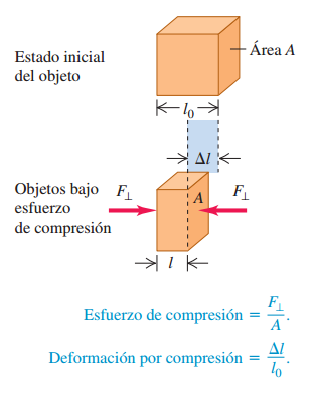
\includegraphics[width=3cm]{../../../../../Pictures/3.jpg}
\\
\caption{Figura 3: Objeto en compresi\'{o}n. El esfuerzo de compresi\'{o}n y la deformaci\'{o}n por compresi\'{o}n se definen igual que en el caso de la tensi\'{o}n (v\'{e}ase la Figura 2), excepto que ahora $\Delta l $ denota la distancia que el objeto se contrae.}
\end{figure 3}\\

\\
El m\'{o}dulo de Young de muchos materiales tiene el mismo valor para esfuerzos de tensi\'{o}n y de compresi\'{o}n; los materiales compuestos como el concreto u hormig\'{o}n son una excepci\'{o}n. Pueden soportar esfuerzo de compresi\'{o}n pero fallan bajo un esfuerzo de tensi\'{o}n comparable. Originalmente en las antiguas civilizaciones como Babilonia, Asiria y Roma, la piedra fue el principal material utilizado ensus estructuras, de modo que \'{e}stas tuvieron que dise\~{n}arse para evitar esfuerzo de tensi\'{o}n. Esto explica el porque tales culturas utilizaron mucho los arcos en entradas y puentes, donde el peso del material que yace encima comprime la piedra y el arco juntos, y no los pone bajo tensi\'{o}n.

\\
\begin{figure 4}
\centering
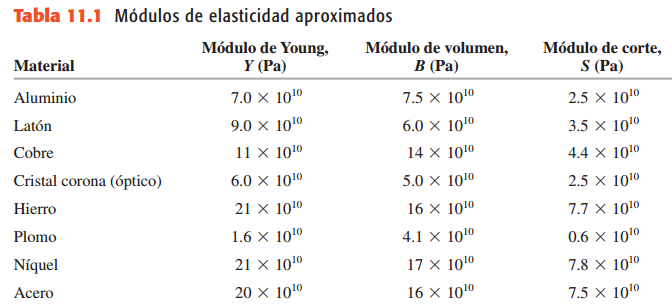
\includegraphics[width=9cm]{../../../../../Pictures/4.jpg}
\\
\caption{Tabla 1: M\'{o}dulos de elasticidad aproximados.}
\end{figure 4}
\\

En muchas situaciones, los cuerpos experimentan esfuerzos de tensi\'{o}n y compresi\'{o}n al mismo tiempo. Por ejemplo, una viga horizontal apoyada en sus extremos se pandea por su propio peso. En consecuencia, la parte superior de la viga est\'{a} en compresi\'{o}n, y la inferior, en tensi\'{o}n (Figura 4.a). Para reducir al m\'{i}nimo el esfuerzo y por ende la deformaci\'{o}n por flexi\'{o}n, la partes superior e inferior de la viga deben tener un \'{a}rea transversal grande. En la l\'{i}nea central de la viga no hay compresi\'{o}n ni tensi\'{o}n, as\'{i} que esta parte puede tener una secci\'{o}n pequea; esto ayuda a reducir al m\'{i}nimo el peso de la viga y tambi\'{e}n a reducir el esfuerzo. El resultado es la viga en I tan utilizada en la construcci\'{o}n de edificios (Figura 4.b).

\\
\begin{figure 5}
\centering
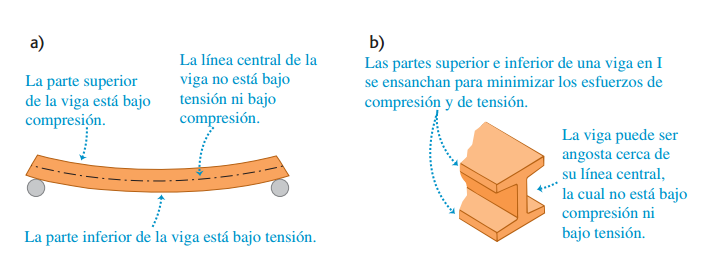
\includegraphics[width=9cm]{../../../../../Pictures/5.jpg}
\\
\caption{Figura 4: a) Una viga apoyada en sus extremos est\'{a} sometida tanto a compresi\'{o}n como a tensi\'{o}n. b) La forma de la secci\'{o}n transversal de una viga en I reduce al m\'{i}nimo tanto el esfuerzo como el peso.}
\end{figure 5}
\\

\textbf{Esfuerzo y deformaci\'{o}n de volumen.}\\ 

Cuando un buzo se sumerge a cierta profundidad en el mar, el agua ejerce una presi\'{o}n
casi uniforme en toda su superficie y reduce un poco su volumen (Figura 1.b). Esta situaci\'{o}n es diferente de los esfuerzos y deformaciones por tensi\'{o}n y compresi\'{o}n que hemos visto. El esfuerzo en este caso es una presi\'{o}n uniforme por todos lados, y la deformaci\'{o}n resultante es un cambio de volumen. Usamos los t\'{e}rminos esfuerzo de volumen y deformaci\'{o}n por volumen para describir estas cantidades.
Si un objeto se sumerge en un fluido (l\'{i}quido o gas) en reposo, el fluido ejerce una
fuerza sobre todas las partes de la superficie del objeto; esta fuerza es perpendicular a
la superficie. (Si trat\'{a}ramos de hacer que el fluido ejerciera una fuerza paralela a la
superficie, el fluido se deslizar\'{i}a a un lado para contrarrestar la acci\'{o}n.) La fuerza $F\bot$ por unidad de \'{a}rea que el fluido ejerce sobre la superficie de un objeto sumergido es la presi\'{o}n p en el fluido:\\

\[P=\frac { F }{ A }\quad(Presi\'{o}n \quad en \quad un \quad fluido)\longrightarrow (5) \]\\


La presi\'{o}n dentro de un fluido aumenta con la profundidad. La presi\'{o}n del aire,
por ejemplo, es aproximadamente 21 porcienrto mayor en el nivel del mar que en Denver (altitud: 1.6 km o 1.0 mi). No obstante, si un objeto sumergido es relativamente peque\~{n}o, podremos ignorar las diferencias de presi\'{o}n debidas a la profundidad en el cuerpo del objeto, en lo que respecta al c\'{a}lculo del esfuerzo de volumen. Por lo tanto, supondremos que la presi\'{o}n tiene el mismo valor para todos los puntos en la superficie del objeto sumergido.La presi\'{o}n tiene las mismas unidades que el esfuerzo; las unidades de uso com\'{u}n incluyen 1 Pa $(={ N }/{ { m }^{ 2 } })$ y $ 1{ lb }/{ { in }^{ 2 }}(1psi)$.\\
\\Tambi\'{e}n se usa com\'{u}nmente la atm\'{o}sfera, que se abrevia atm. Una atm\'{o}sfera es la presi\'{o}n media aproximada de la atm\'{o}sfera terrestre al nivel del mar:\\

\[1\quad Atm\'{o}sfeta= 1\quad atm = 1.013{ \times 10 }^{ 5 }Pa=14.7 { \quad lb }/{ { in }^{ 2 } }\]
\\ 
\textbf{CUIDADO} Presi\'{o}n contra fuerza a diferencia de la fuerza, la presi\'{o}n no tiene una direcci\'{o}n intr\'{i}nseca: la presi\'{o}n en la superficie de un objeto sumergido es la misma, sea cual fuere la orientaci\'{o}n de la superficie. Por lo tanto, la presi\'{o}n es una cantidad escalar, no vectorial. La presi\'{o}n desempe\~{n}a el papel del esfuerzo en un cambio de volumen. La deformaci\'{o}n correspondiente es el cambio fraccionario en el volumen(Figura 6), es decir, el cociente del cambio de volumen $\Delta V$ entre el volumen original Vo:
\\

\[Deformaci\'{o}n\quad por\quad volumen=\frac { \Delta V }{ Vo }\longrightarrow(6) \]

La deformaci\'{o}n por volumen es el cambio de volumen por unidad de volumen. Al igual que la deformaci\'{o}n por tensi\'{o}n o compresi\'{o}n, es un n\'{u}mero puro, sin unidades. Si se obedece la ley de Hooke, un aumento en la presi\'{o}n (esfuerzo de volumen) produce una deformaci\'{o}n por volumen (cambio fraccionario de volumen) proporcional. 
\\
\\
\begin{figure 6}
\centering
\\
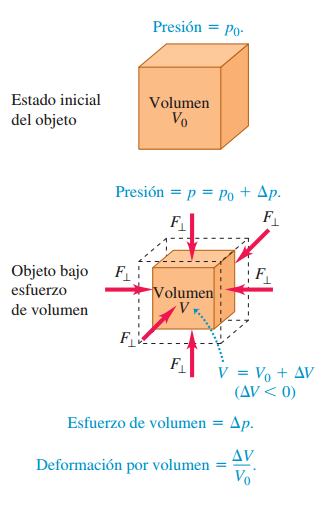
\includegraphics[width=5cm]{../../../../../Pictures/6.jpg}
\\
\caption{Figura 6: Objeto sometido a un esfuerzo de volumen. Sin el esfuerzo, el cubo ocupa un volumen Vo; cuando se aplica el esfuerzo, el cubo tiene un volumen menor, V. Por claridad, se exager\'{o} el cambio de volumen $\Delta V$.}
\end{figure 6}
\\
\\
El m\'{o}dulo de elasticidad correspondiente (relaci\'{o}n esfuerzo-deformaci\'{o}n) se denomina \textbf{m\'{o}dulo de volumen} y se denota con B. Si la presi\'{o}n sobre un cuerpo cambia en una cantidad peque\~{n}a $\Delta P$, de P0 a P0 + $\Delta V$ y la deformaci\'{o}n por volumen resultante es $\frac { -\Delta V }{ Vo }$, la ley de Hooke adopta la forma:\\

\[B=\frac { Esfuerzo\quad de\quad \quad volumen }{ Deformaci\'{o}n\quad por\quad volumen } =-\frac { \Delta p }{ \sfrac { \Delta V }{ Vo }  } \quad (M\'{o}dulo\quad de\quad Volumen)\longrightarrow(7)\]

Incluimos un signo de menos en esta ecuaci\'{o}n porque un aumento de presi\'{o}n siempre
causa una reducci\'{o}n de volumen. En otras palabras, si $\Delta P$ es positivo, $\Delta V$ es negativo. El m\'{o}dulo de volumen B en s\'{i} es una cantidad positiva. En el caso de cambios de presi\'{o}n peque\~{n}os en un s\'{olido o un l\'{i]quido, consideramos que B es constante. El m\'{o}dulo de volumen de un gas, sin embargo, depende de la presi\'{o}n inicial Po. La Tabla 1 da valores del m\'{O}dulo de volumen para varios materiales s\'{O}lidos. Sus unidades, fuerza por unidad de \'{a}rea, son las de la presi\'{o}n (las mismas del esfuerzo de tensi\'{o}n o compresi\'{o}n).

Un objeto sometido a un esfuerzo de volumen. Sin el esfuerzo, el cubo ocupa un volumen Vo; cuando se aplica el esfuerzo, el cubo tiene un volumen menor, V. Por claridad, se exager{o} el cambio de volumen $\Delta V$ Esfuerzo, deformaci\'{o}n y m\'{o}dulos de elasticidad. El rec\'{o}proco del m\'{o}dulo de volumen se denomina compresibilidad y se denota con k. Por la ecuaci\'{o}n (7): 
\\
\[k=\frac { 1 }{ B } =-\frac { { \Delta V }/{ Vo } }{ \Delta P } =-\frac { 1 }{ Vo } \frac { \Delta V }{ \Delta P } \quad (Compresibilidad)\longrightarrow (8)\]

La compresibilidad es la disminuci\'{o}n fraccionaria de volumen,${ -\Delta V }/{ Vo }$ , por unidad de aumento p de la presi\'{o}n. Las unidades de la compresibilidad son inversas a las de presi\'{o}n, ${ Pa }^{ -1 }$ o ${ atm }^{ -1 }$. La compresibilidad del agua, por ejemplo, es de $46.4\times { 10 }^{ -6 }{ atm }^{ -1 }$. Esto implica que, por cada aumento de 1 atm en la presi\'{o}n, el volumen del agua disminuye en 46.4 partes por mill\'{o}n. Los materiales con m\'{o}dulo de volumen peque\~{n}o y compresibilidad grande son f\'{a}ciles de comprimir.\\


\textbf{Esfuerzo y deformaci\'{o}n por corte.}\\

\\El tercer tipo de situaci\'{o}n de esfuerzo-deformaci\'{o}n se denomina corte. El list\'{o}n de la Figura 1.c est\'{a} sometido a un \textbf{esfuerzo de corte}: una parte del list\'{o}n se est\'{a} empujando hacia arriba, mientras una parte adyacente se est\'{a} empujando hacia abajo, lo que produce un cambio de forma del list\'{o}n. La Figura 7 muestra un cuerpo deformado por un esfuerzo de corte.\\

\begin{figure 7}
\centering
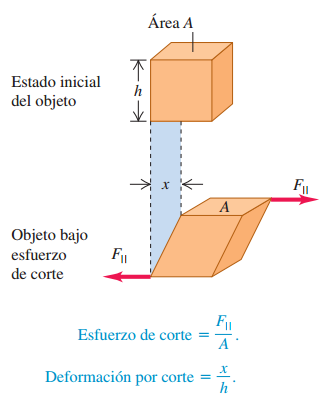
\includegraphics[width=4cm]{../../../../../Pictures/7.png}
\\
\caption{Figura 7: Objeto sometido a un esfuerzo de corte. Se aplican fuerzas tangentes a superficies opuestas del objeto (en contraste con la situaci\'{o}n de la Figura 2, donde las fuerzas act\'{u}an perpendiculares a las superficies).Por claridad, se exagera la deformaci\'{o}n x.}
\end{figure 7}\\

\\
\\
\\En la figura, fuerzas de igual magnitud pero direcci\'{o}n opuesta act\'{u}an de forma tangente a las superficies de extremos opuestos del objeto. Definimos el esfuerzo de corte como la fuerza $F\Vert$ que act\'{u}a tangente a la superficie, dividida entre el \'{a}rea A sobre la que act\'{u}a:\\

\[Esfuerzo\quad de\quad corte=\frac { F }{ A }\longrightarrow (9)\]
\\

Al igual que los otros dos tipos de esfuerzo, el esfuerzo de corte es una fuerza por
unidad de \'{a}rea. La figura 7 muestra que una cara del objeto sometido a esfuerzo de corte se
desplaza una distancia x relativa a la cara opuesta. Definimos la \textbf{deformaci\'{o}n por
corte} como el cociente del desplazamiento x entre la dimensi\'{o}n transversal h:\\

\[Deformaci\'{o}n\quad por\quad corte=\frac { x }{ h}\longrightarrow (10)\] \\

En situaciones reales, x casi siempre es mucho menor que h. Como todas las deformaciones, la deformaci\'{o}n por corte es un n\'{u}mero adimensional: un cociente de dos longitudes. Si las fuerzas son lo suficientemente peque\~{n}as como para que se obedezca la ley de Hooke, la deformaci\'{o}n por corte es proporcional al esfuerzo de corte. El m\'{o}dulo de elasticidad correspondiente(cociente del esfuerzo de corte entre la deformaci\'{o}n por corte) se denomina m\'{o}dulo de corte y se denota con S:\\


\[S=\frac { Esfuerzo\quad de\quad corte }{ Deformaci\'{o}n\quad por\quad corte } =\frac { { F }/{ A } }{ { x }/{ h } } =\frac { F }{ A } \frac { h }{ x } \quad (m\'{o}dulo\quad de\quad corte)\longrightarrow (11)\]\\

Para un material dado, S suele ser de un tercio a un medio del valor del m\'{o}dulo de Young Y para el esfuerzo de tensi\'{o}n. Tenga en cuenta que los conceptos de esfuerzo de corte, deformaci\'{o}n por corte y m\'{o}dulo de corte \'{u}nicamente se aplican a materiales s\'{o}lidos. La raz\'{o}n es que
las fuerzas de corte deben deformar el bloque s\'{o}lido, el cual tiende a regresar a su forma original si se eliminan las fuerzas de corte. En cambio, los gases
y l\'{i}quidos no tienen forma definida.
\section{Desarrollo Experimental.}\\
\textbf{Materiales:} 
Soporte con material \'{o}ptico reflexivo (espejo y rayo de luz).\\
Material a estudiar (lat\'{o}n o cobre). \\
Hoja de papel milim\'{e}trico. \\
Regla y l\'{a}piz. \\
Fuente de alimentaci\'{o}n.\\
Pesas de distintas masas. \\
Metro para medir. \\
Nivel de agua. \\
Medidor de ángulos de inclinaci\'{o}n \\
\\
\\
\textbf{M\'{e}todo 1. Procedimiento:} \\
Comenzamos la pr\'{a}ctica con el material proporcionado por el equipo de laboratorio, procedimos a medir algunas de nuestras constantes como lo son; la distancia del soporte medida desde el espejo hasta la hoja de papel milim\'{e}trico (X), la elongaci\'{o}n inicial del material ya sea lat\'{o}n o cobre, la distancia del soporte para en espejo hasta el hilo, y procedimos a medir el \'{a}rea transversal del material por medio de un tornillo microm\'{e}trico. 

\end{document}